\PassOptionsToPackage{unicode=true}{hyperref} % options for packages loaded elsewhere
\PassOptionsToPackage{hyphens}{url}
\documentclass[11pt,dvipsnames,ignorenonframetext,aspectratio=169]{beamer}
\IfFileExists{pgfpages.sty}{\usepackage{pgfpages}}{}
\setbeamertemplate{caption}[numbered]
\setbeamertemplate{caption label separator}{: }
\setbeamercolor{caption name}{fg=normal text.fg}
\beamertemplatenavigationsymbolsempty
\usepackage{lmodern}
\usepackage{amssymb,amsmath}
\usepackage{ifxetex,ifluatex}
\usepackage{fixltx2e} % provides \textsubscript
\ifnum 0\ifxetex 1\fi\ifluatex 1\fi=0 % if pdftex
  \usepackage[T1]{fontenc}
  \usepackage[utf8]{inputenc}
\else % if luatex or xelatex
  \ifxetex
    \usepackage{mathspec}
  \else
    \usepackage{fontspec}
\fi
\defaultfontfeatures{Ligatures=TeX,Scale=MatchLowercase}







\fi

  \usetheme[]{monash}

  \usecolortheme{monashwhite}


% A default size of 24 is set in beamerthememonash.sty

% Title page
\setbeamertemplate{title page}
{\placefig{-0.01}{-0.01}{width=1.01\paperwidth,height=1.01\paperheight}{rhinocerousbeetle.jpg}
% \begin{textblock}{7.5}(1,2.8)\usebeamerfont{title} % original
\begin{textblock}{15}(1,2.2)\usebeamerfont{title}
{\color{white}\raggedright\par\inserttitle}
\end{textblock}
\begin{textblock}{10}(1,6)
\small
{\color{white}\raggedright{\insertauthor}\mbox{}\\[0.1cm]
\insertdate}
\end{textblock}}


  \useinnertheme{rounded}

  \useoutertheme{smoothtree}

% use upquote if available, for straight quotes in verbatim environments
\IfFileExists{upquote.sty}{\usepackage{upquote}}{}
% use microtype if available
\IfFileExists{microtype.sty}{%
  \usepackage{microtype}
  \UseMicrotypeSet[protrusion]{basicmath} % disable protrusion for tt fonts
}{}


\newif\ifbibliography


\hypersetup{
      pdftitle={Chromosome and genetic control mechanism in eukaryotes},
            colorlinks=true,
    linkcolor=red,
    citecolor=Blue,
    urlcolor=lightgrayd,
    breaklinks=true}
%\urlstyle{same}  % Use monospace font for urls







% Prevent slide breaks in the middle of a paragraph:
\widowpenalties 1 10000
\raggedbottom

  \AtBeginPart{
    \let\insertpartnumber\relax
    \let\partname\relax
    \frame{\partpage}
  }
  \AtBeginSection{
    \ifbibliography
    \else
      \let\insertsectionnumber\relax
      \let\sectionname\relax
      \frame{\sectionpage}
    \fi
  }
  \AtBeginSubsection{
    \let\insertsubsectionnumber\relax
    \let\subsectionname\relax
    \frame{\subsectionpage}
  }



\setlength{\parindent}{0pt}
\setlength{\parskip}{6pt plus 2pt minus 1pt}
\setlength{\emergencystretch}{3em}  % prevent overfull lines
\providecommand{\tightlist}{%
  \setlength{\itemsep}{0pt}\setlength{\parskip}{0pt}}

  \setcounter{secnumdepth}{0}


%% Monash overrides
\AtBeginSection[]{
   \frame<beamer>{
   \frametitle{Outline}\vspace*{0.2cm}
   
   \tableofcontents[currentsection,hideallsubsections]
  }}

% Redefine shaded environment if it exists (to ensure text is black)
\ifcsname Shaded\endcsname
  \definecolor{shadecolor}{RGB}{225,225,225}
  \renewenvironment{Shaded}{\color{black}\begin{snugshade}\color{black}}{\end{snugshade}}
\fi
%%

  \usepackage{setspace}
  \usepackage{wasysym}
  % \usepackage{footnote} % don't use this this breaks all
  \usepackage{fontenc}
  \usepackage{fontawesome}
  \usepackage{booktabs,siunitx}
  \usepackage{longtable}
  \usepackage{array}
  \usepackage{multirow}
  \usepackage{wrapfig}
  \usepackage{float}
  \usepackage{colortbl}
  \usepackage{pdflscape}
  \usepackage{tabu}
  \usepackage{threeparttable}
  \usepackage{threeparttablex}
  \usepackage[normalem]{ulem}
  \usepackage{makecell}
  \usepackage{xcolor}
  \usepackage{tikz} % required for image opacity change
  \usepackage[absolute,overlay]{textpos} % for text formatting
  \usepackage{chemfig}
  \usepackage[skip=0.333\baselineskip]{caption}
  % \newcommand*{\AlignChar}[1]{\makebox[1ex][c]{\ensuremath{\scriptstyle#1}}}%

  % this font option is amenable for beamer
  \setbeamerfont{caption}{size=\tiny}
  \singlespacing
  \definecolor{lightgrayd}{gray}{0.95}
  \definecolor{skyblued}{rgb}{0.65, 0.6, 0.94}
  \definecolor{oranged}{RGB}{245, 145, 200}

  \newlength{\cslhangindent}
  \setlength{\cslhangindent}{1.5em}
  \newenvironment{cslreferences}%
    {\setlength{\parindent}{0pt}%
    \everypar{\setlength{\hangindent}{\cslhangindent}}\ignorespaces}%
    {\par}

  \title[]{Chromosome and genetic control mechanism in eukaryotes}


  \author[
        Deependra Dhakal\\
College of Natural Resource Management\\
Agriculture and Forestry University\\
\textit{ddhakal.rookie@gmail.com}\\
\url{https://rookie.rbind.io}
    ]{Deependra Dhakal\\
College of Natural Resource Management\\
Agriculture and Forestry University\\
\textit{ddhakal.rookie@gmail.com}\\
\url{https://rookie.rbind.io}}


\date[
      
  ]{
    }

\begin{document}

% Hide progress bar and footline on titlepage
  \begin{frame}[plain]
  \titlepage
  \end{frame}


   \frame<beamer>{
   \frametitle{Outline}\vspace*{0.2cm}
   
   \tableofcontents[hideallsubsections]
  }

\hypertarget{eukaryotic-chromosome}{%
\section{Eukaryotic chromosome}\label{eukaryotic-chromosome}}

\begin{frame}{}
\protect\hypertarget{section}{}
\begin{itemize}
\tightlist
\item
  One notable difference between eukaryotic and prokaryotic DNA is that
  eukaryotic DNA is packaged into nucleosomes, forming
  \textbf{chromatin} leading to an ultimate assemblage structure called,
  chromosome whereas bacterial DNA lacks nucleosomes.
\item
  In eukaryotes, chromatin structure is dynamic and is an essential
  ingredient in gene regulation.
\item
  The chromosome complement in a cell nucleus in the members of a
  species is called their \textbf{karyotype} (records all the
  cytologically identifiable chromosome features (size, form, number)).
\end{itemize}
\end{frame}

\begin{frame}{}
\protect\hypertarget{section-1}{}
\begin{itemize}
\tightlist
\item
  The number of identical chromosome sets in a cell nucleus determines
  the level of ploidy, \emph{n}.
\item
  Cell nuclei with only one set of chromosomes are haploid ( \emph{1n};
  Greek \emph{haplos}, simple) somatic (tissue) cells are predominantly
  diploid ( \emph{2n}) in ferns and seed plants.
\item
  Gametic chromosome number = 1/2 x Somatic chromosome number
\item
  Two copies of a chromosome are ordinarily identical in morphology,
  gene content and gene order; they are called \textbf{homologous
  chromosomes}.
\item
  The \textbf{C value} refers to the total amount of DNA in the haploid
  genome, given in picograms.
\item
  The C value of the bacterium Escherichia coli is 0.004, that of
  tobacco is 1.6, that of maize is 7.5, and that of some lily species
  can be over 30.
\end{itemize}
\end{frame}

\begin{frame}{}
\protect\hypertarget{section-2}{}
\begin{itemize}
\tightlist
\item
  The following chromosome features are particularly important: (Figure
  \ref{fig:chromosome-structure}) length, position of the centromere,
  presence or absence of a nucleolar organizing region (NOR), and
  heterochromatic sections.
\item
  Each metaphase chromosome appears to be longitudinally divided into
  two identical parts each of which is known as \textbf{chromatid}, a
  single is reffered to as sister chromatid.
\item
  The centromere (primary constriction; Greek kentron, middle point and
  meros, part) is the narrowest point on the chromosome, where the
  chromosome bends during chromosome movements in cell division and
  where the microtubules of the nuclear spindle attach.
\item
  The part of a chromatid on either side of the centromere is referred
  to as an arm of the chromatid, characterized by \textbf{centromere
  index}. (An uncondensed, unduplicated chromosome has a single
  centromere and two arms.)
\item
  Based on the relative position of centromere on chromosomes, they can
  be: Metacentric, Submetacentric, Acrocentric, Telocentric
\end{itemize}
\end{frame}

\begin{frame}{}
\protect\hypertarget{section-3}{}
\begin{itemize}
\tightlist
\item
  Centromeric region of chromosome contains satellite DNA.
\item
  Telomeric region of chromosome is highly stable and has DNA loops.
\item
  The chromosome region lying between secondary constriction and the
  nearest telomere is known as satellite. Therefore chromosomes having
  secondary constrictions are called satellite chromosomes.
\item
  Nucleolus is always associated with the secondary constrictions of
  sat-chromosomes, thus these constrictions are sometimes also called
  NOR.
\item
  In some species e.g., maize, amphibia etc, chromosomes during first
  prophase of meiosis (pachytene), show small bead-like structures
  called chromomeres.
\item
  Homologous chromosomes always show identical pattern of chromomere
  distribution.
\end{itemize}
\end{frame}

\begin{frame}{}
\protect\hypertarget{section-4}{}
\begin{figure}
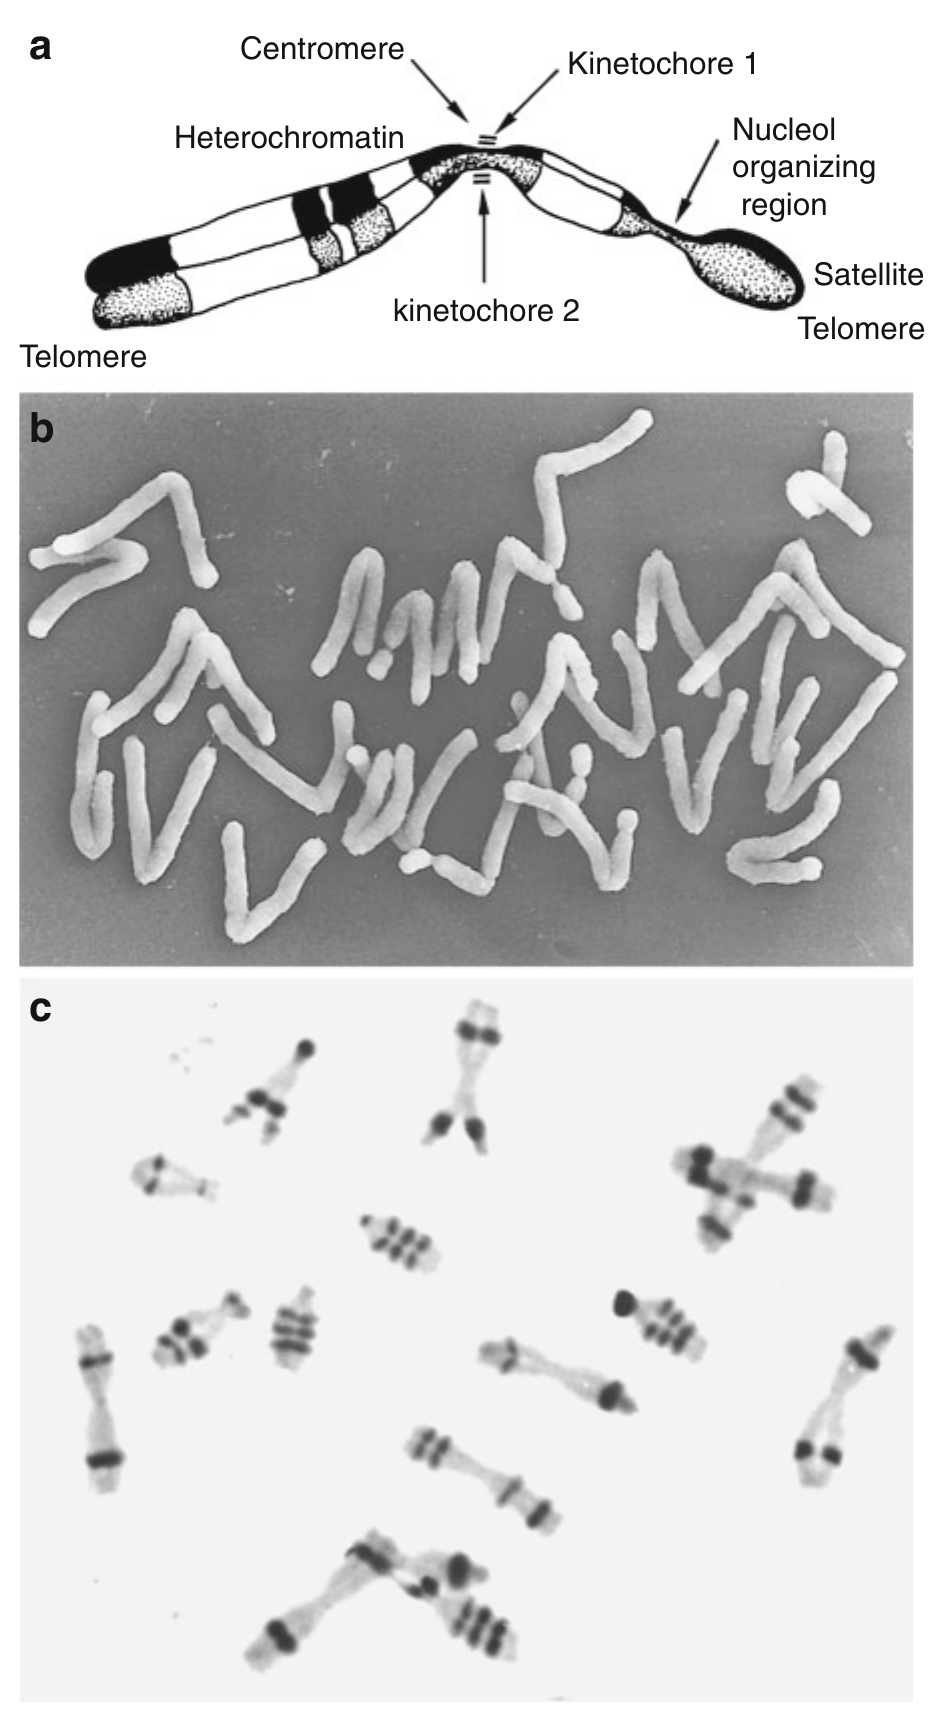
\includegraphics[width=0.22\linewidth]{../images/chromosome_structure} \caption{Chromosomes occur as compact entities during nuclear division (e.g., in metaphase and anaphase of mitosis). This entity is what was originally named 'chromosome.' (a) A satellite chromosome with the two telomeres, the centromere with the two kinetochores (insertion points of the microtubules on the spindle apparatus), heterochromatic bands (additional regions on the telomeres and in the region of the centromere), and the characteristic (for satellite chromosomes) nucleolar organizing region (NOR) and a heterochromatic satellite. The chromosome is split longitudinally into two chromatids that later become daughter chromosomes. (b) Anaphase chromosomes of barley (Hordeum vulgare) with a diploid chromosome number 2n = 28, two satellite chromosomes per complement. The four NORs and four satellites of the two complements of daughter chromosomes can be seen clearly (x1,880). (c) Chromosome complement of \textit{Anemone blanda} (2n = 16); heterochromatic bands (except at the centromere) picked out with color (x600)}\label{fig:chromosome-structure}
\end{figure}
\end{frame}

\begin{frame}{Chromosome numbers}
\protect\hypertarget{chromosome-numbers}{}
\begin{table}

\caption{\label{tab:chromosome-number1}Chromosome numbers found different species of organisms (animals)}
\centering
\fontsize{6}{8}\selectfont
\begin{tabular}[t]{>{\raggedright\arraybackslash}p{8em}>{\raggedright\arraybackslash}p{12em}>{\raggedright\arraybackslash}p{8em}>{\raggedright\arraybackslash}p{8em}>{\raggedright\arraybackslash}p{12em}>{\raggedright\arraybackslash}p{8em}}
\toprule
Common name & Species & Diploid number & Common name & Species & Diploid number\\
\midrule
\cellcolor{gray!6}{Man} & \cellcolor{gray!6}{$\textit{Homo sapiens}$} & \cellcolor{gray!6}{46} & \cellcolor{gray!6}{Alligator} & \cellcolor{gray!6}{$\textit{Alligator mississipiensis}$} & \cellcolor{gray!6}{32}\\
Chimpanzee & $\textit{Pan troglodytes}$ & 48 & Toad & $\textit{Bufo americanus}$ & 22\\
\cellcolor{gray!6}{Gorilla} & \cellcolor{gray!6}{$\textit{Gorilla gorilla}$} & \cellcolor{gray!6}{48} & \cellcolor{gray!6}{Frog} & \cellcolor{gray!6}{$\textit{Rana pipiens}$} & \cellcolor{gray!6}{26}\\
Rhesus monkey & $\textit{Macaca mulatta}$ & 42 & Carp & $\textit{Cyprinus carpio}$ & 104\\
\cellcolor{gray!6}{Cattle} & \cellcolor{gray!6}{$\textit{Bos taurus}$} & \cellcolor{gray!6}{60} & \cellcolor{gray!6}{Starfish} & \cellcolor{gray!6}{$\textit{Asterias forbesi}$} & \cellcolor{gray!6}{36}\\
\addlinespace
Dog & $\textit{Canis familaris}$ & 78 & Silkworm & $\textit{Bombyx mori}$ & 56\\
\cellcolor{gray!6}{Cattle} & \cellcolor{gray!6}{$\textit{Felis domesticus}$} & \cellcolor{gray!6}{38} & \cellcolor{gray!6}{Red ant} & \cellcolor{gray!6}{$\textit{Formica sanguinea}$} & \cellcolor{gray!6}{48}\\
Horse & $\textit{Equus calibus}$ & 64 & House fly & $\textit{Musca domestica}$ & 12\\
\cellcolor{gray!6}{Donkey} & \cellcolor{gray!6}{$\textit{Equus asinus}$} & \cellcolor{gray!6}{62} & \cellcolor{gray!6}{Fruit fly} & \cellcolor{gray!6}{$\textit{Drosophila melanogaster}$} & \cellcolor{gray!6}{8}\\
House mouse & $\textit{Mus musculus}$ & 40 & Mosquito & $\textit{Culex pipiens}$ & 6\\
\addlinespace
\cellcolor{gray!6}{Rat} & \cellcolor{gray!6}{$\textit{Rattus norvegicus}$} & \cellcolor{gray!6}{42} & \cellcolor{gray!6}{Cockroach} & \cellcolor{gray!6}{$\textit{Blatta germanica}$} & \cellcolor{gray!6}{23 $\male$, 24 $\female$}\\
Golden hampster & $\textit{Mesocrietus auratus}$ & 44 & Grasshopper & $\textit{Melanoplus differentialis}$ & 24\\
\cellcolor{gray!6}{Guinea pig} & \cellcolor{gray!6}{$\textit{Cavia cobaya}$} & \cellcolor{gray!6}{64} & \cellcolor{gray!6}{Honeybee} & \cellcolor{gray!6}{$\textit{Apis mellifera}$} & \cellcolor{gray!6}{32}\\
Rabbit & $\textit{Orychtolagus cuniculus}$ & 44 & Flatworm & $\textit{Planaria torva}$ & 16\\
\cellcolor{gray!6}{Pigeon} & \cellcolor{gray!6}{$\textit{Columbia livia}$} & \cellcolor{gray!6}{80} & \cellcolor{gray!6}{Freshwater hydra} & \cellcolor{gray!6}{$\textit{Hydra vulgaria attenuata}$} & \cellcolor{gray!6}{32}\\
\addlinespace
Chicken & $\textit{Gallus domesticus}$ & 78 & Nematode & $\textit{Caenorhabditis elegans}$ & 11 $\male$, 12 $\female$\\
\bottomrule
\end{tabular}
\end{table}
\end{frame}

\begin{frame}{}
\protect\hypertarget{section-5}{}
\begin{columns}[T,onlytextwidth]
  
  \column{0.4\textwidth}

\begin{table}

\caption{\label{tab:chromosome-number2}Chromosome numbers found different species of organisms (Other organisms; haploid chromosome number)}
\centering
\fontsize{6}{8}\selectfont
\begin{tabular}[t]{>{\raggedright\arraybackslash}p{4em}>{\raggedright\arraybackslash}p{8em}>{\raggedright\arraybackslash}p{4em}}
\toprule
Common name & Species & Haploid number\\
\midrule
\cellcolor{gray!6}{Yeast} & \cellcolor{gray!6}{$\textit{Saccharomyces cerevisiae}$} & \cellcolor{gray!6}{17}\\
Slime mold & $\textit{Dictyostelium discoideum}$ & 7\\
\cellcolor{gray!6}{Black bread mold} & \cellcolor{gray!6}{$\textit{Aspergillus nidulans}$} & \cellcolor{gray!6}{8}\\
Pink bread mold & $\textit{Neurospora crassa}$ & 7\\
\cellcolor{gray!6}{Penicillin mold} & \cellcolor{gray!6}{$\textit{Penicillium species}$} & \cellcolor{gray!6}{4}\\
\addlinespace
Green algae & $\textit{Chlamydomonas reinhardtii}$ & 16\\
\cellcolor{gray!6}{Amoeba} & \cellcolor{gray!6}{$\textit{Amoeba proteus}$} & \cellcolor{gray!6}{250}\\
\bottomrule
\end{tabular}
\end{table}

  \column{0.6\textwidth}

\begin{table}

\caption{\label{tab:chromosome-number3}Chromosome numbers found different species of organisms (Plants)}
\centering
\fontsize{5}{7}\selectfont
\begin{tabular}[t]{>{\raggedright\arraybackslash}p{4em}>{\raggedright\arraybackslash}p{8em}>{\raggedright\arraybackslash}p{4em}>{\raggedright\arraybackslash}p{4em}>{\raggedright\arraybackslash}p{8em}>{\raggedright\arraybackslash}p{4em}}
\toprule
Common name & Species & Diploid number & Common name & Species & Diploid number\\
\midrule
\cellcolor{gray!6}{Green algae} & \cellcolor{gray!6}{$\textit{Acetabularia mediterranea}$} & \cellcolor{gray!6}{20} & \cellcolor{gray!6}{Tomato} & \cellcolor{gray!6}{$\textit{Lycopersicon esculentum}$} & \cellcolor{gray!6}{24}\\
Garden onion & $\textit{Allium cepa}$ & 16 & Tobacco & $\textit{Nicotiana tabacum}$ & 48\\
\cellcolor{gray!6}{Barley} & \cellcolor{gray!6}{$\textit{Hordeum vulgare}$} & \cellcolor{gray!6}{14} & \cellcolor{gray!6}{Evening primerose} & \cellcolor{gray!6}{$\textit{Oenothera biennis}$} & \cellcolor{gray!6}{14}\\
Rice & $\textit{Oryza sativa}$ & 24 & Kidney bean & $\textit{Phaseolus vulgaris}$ & 22\\
\cellcolor{gray!6}{Spiderwort} & \cellcolor{gray!6}{$\textit{Tradescantia vairginiana}$} & \cellcolor{gray!6}{24} & \cellcolor{gray!6}{White oak} & \cellcolor{gray!6}{$\textit{Quercus alba}$} & \cellcolor{gray!6}{24}\\
\addlinespace
Wheat & $\textit{Triticum aestivum}$ & 42 & Pine & $\textit{Pinus species}$ & 24\\
\cellcolor{gray!6}{Corn (maize)} & \cellcolor{gray!6}{$\textit{Zea mays}$} & \cellcolor{gray!6}{20} & \cellcolor{gray!6}{Garden pea} & \cellcolor{gray!6}{$\textit{Pisum sativum}$} & \cellcolor{gray!6}{14}\\
Snapdragon & $\textit{Antirrhinum majus}$ & 16 & Potato & $\textit{Solanum tuberosum}$ & 48\\
\cellcolor{gray!6}{Squash} & \cellcolor{gray!6}{$\textit{Cucurbita pepo}$} & \cellcolor{gray!6}{40} & \cellcolor{gray!6}{White clover} & \cellcolor{gray!6}{$\textit{Trifolium repens}$} & \cellcolor{gray!6}{32}\\
Upland cotton & $\textit{Gossypium hirsutum}$ & 52 & Broad bean & $\textit{Vicia faba}$ & 12\\
\bottomrule
\end{tabular}
\end{table}

\end{columns}
\end{frame}

\begin{frame}{Distribution of chromosomes during eukaryotic cell
division}
\protect\hypertarget{distribution-of-chromosomes-during-eukaryotic-cell-division}{}
\begin{itemize}
\tightlist
\item
  When a cell is not dividing, and even as it replicates its DNA in
  preparation for cell division, each chromosome is in the form of a
  long, thin chromatin fiber.
\item
  After DNA replication, however, the chromosomes condense as a part of
  cell division: Each chromatin fiber becomes densely coiled and folded,
  making the chromosomes much shorter and so thick that we can see them
  with a light microscope.
\item
  Each duplicated chromosome has two sister chromatids, which are joined
  copies of the original chromosome (Figure
  \ref{fig:duplicated-chromosome}).
\item
  The two chromatids, each containing an identical DNA molecule, are
  initially attached all along their lengths by protein complexes called
  cohesins.
\end{itemize}
\end{frame}

\begin{frame}{}
\protect\hypertarget{section-6}{}
\begin{itemize}
\tightlist
\item
  Each sister chromatid has a centromere, a region containing specific
  DNA sequences where the chromatid is attached most closely to its
  sister chromatid. This attachment is mediated by protein bound to the
  centromeric DNA sequences and gives the condensed, duplicated
  chromosome a narrow ``waist''.
\item
  Later in the cell division process, the two sister chromatids of each
  duplicated chromosomes separate and move into two new nuclei, one
  forming at each end of the cell. Once they separate they are
  considered individual chromosomes.
\end{itemize}
\end{frame}

\begin{frame}{}
\protect\hypertarget{section-7}{}
\begin{figure}

{\centering 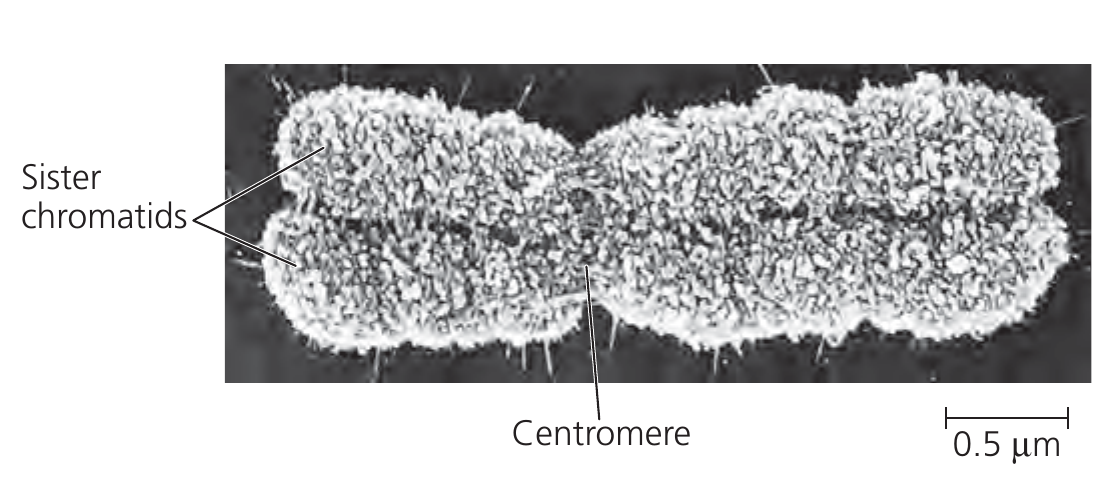
\includegraphics[width=0.8\linewidth]{../images/duplicated_chromosomes_hd} 

}

\caption{Sister chromatids held together along their length by 'cohesin' proteins.}\label{fig:duplicated-chromosome}
\end{figure}
\end{frame}

\hypertarget{chromatin}{%
\section{Chromatin}\label{chromatin}}

\begin{frame}{}
\protect\hypertarget{section-8}{}
\small

\begin{itemize}
\tightlist
\item
  Most of the nuclear DNA is complexed with histones.
\item
  Histones are characteristic to eukaryotes (except dinoflagellates)
\item
  The mass ratio of histone to DNA is about 1:1.
\item
  Histones only occur together with DNA in living cells.
\item
  They are synthesized synchronously with the DNA in the replication
  phase of the cell cycle (S phase) in the cytoplasm and are immediately
  transferred to the cell nucleus.
\item
  The strongly acidic DNA acts as a polyanion and attracts the histone
  molecule, which is basic as a result of its many lysine and arginine
  residues (pI about 12) and acts as a polycation.
\item
  The H1--H4 (Given in Table \ref{fig:histone-types}) series is ordered
  according to the decreasing proportion of lysine and the increasing
  proportion of arginine. The histones, especially H3 and H4, have
  altered little during phylogenesis.
\end{itemize}
\end{frame}

\begin{frame}{Heterochromatin and euchromatin}
\protect\hypertarget{heterochromatin-and-euchromatin}{}
\begin{itemize}
\tightlist
\item
  Based on stainability of chromatin chromosomes can be Heterochromatin
  and Euchromatin.
\item
  This is due to variation in density of chromatin.
\item
  Euchromatin takes up little stain during interphase, stains only
  lightly during prophase, but is deeply stained during metaphase.
\item
  Heterochromatin takes up deep stain during interphase and prophase,
  while during metaphase it is stained lightly.
\item
  In general heterochromatin is found in the centromeric and telomeric
  regions.
\item
  Almost all of the genes of eukaryotes in a chromosomes are found in
  euchromatin region.
\end{itemize}
\end{frame}

\begin{frame}{}
\protect\hypertarget{section-9}{}
\begin{itemize}
\tightlist
\item
  Moreover, when euchromatic genes are artificially transposed to a
  heterochromatic environment, they tend to function abnormally, and, in
  some cases, they do not to function at all.
\item
  This impaired ability to function can create a mixture of normal and
  mutant characteristics in the same individual, a condition referred to
  as \textbf{position-effect variegation}.
\item
  This term is used because the variability in the phenotype is caused
  by changing the position of the euchromatic gene, specifically by
  relocating it to the heterochromatin.
\item
  Many examples of position-effect variegation have been discovered in
  Drosophila, usually in association with inversion or translocations
  that move a euchromatic gene into the heterochromatin.
\end{itemize}
\end{frame}

\begin{frame}{}
\protect\hypertarget{section-10}{}
\begin{figure}

{\centering 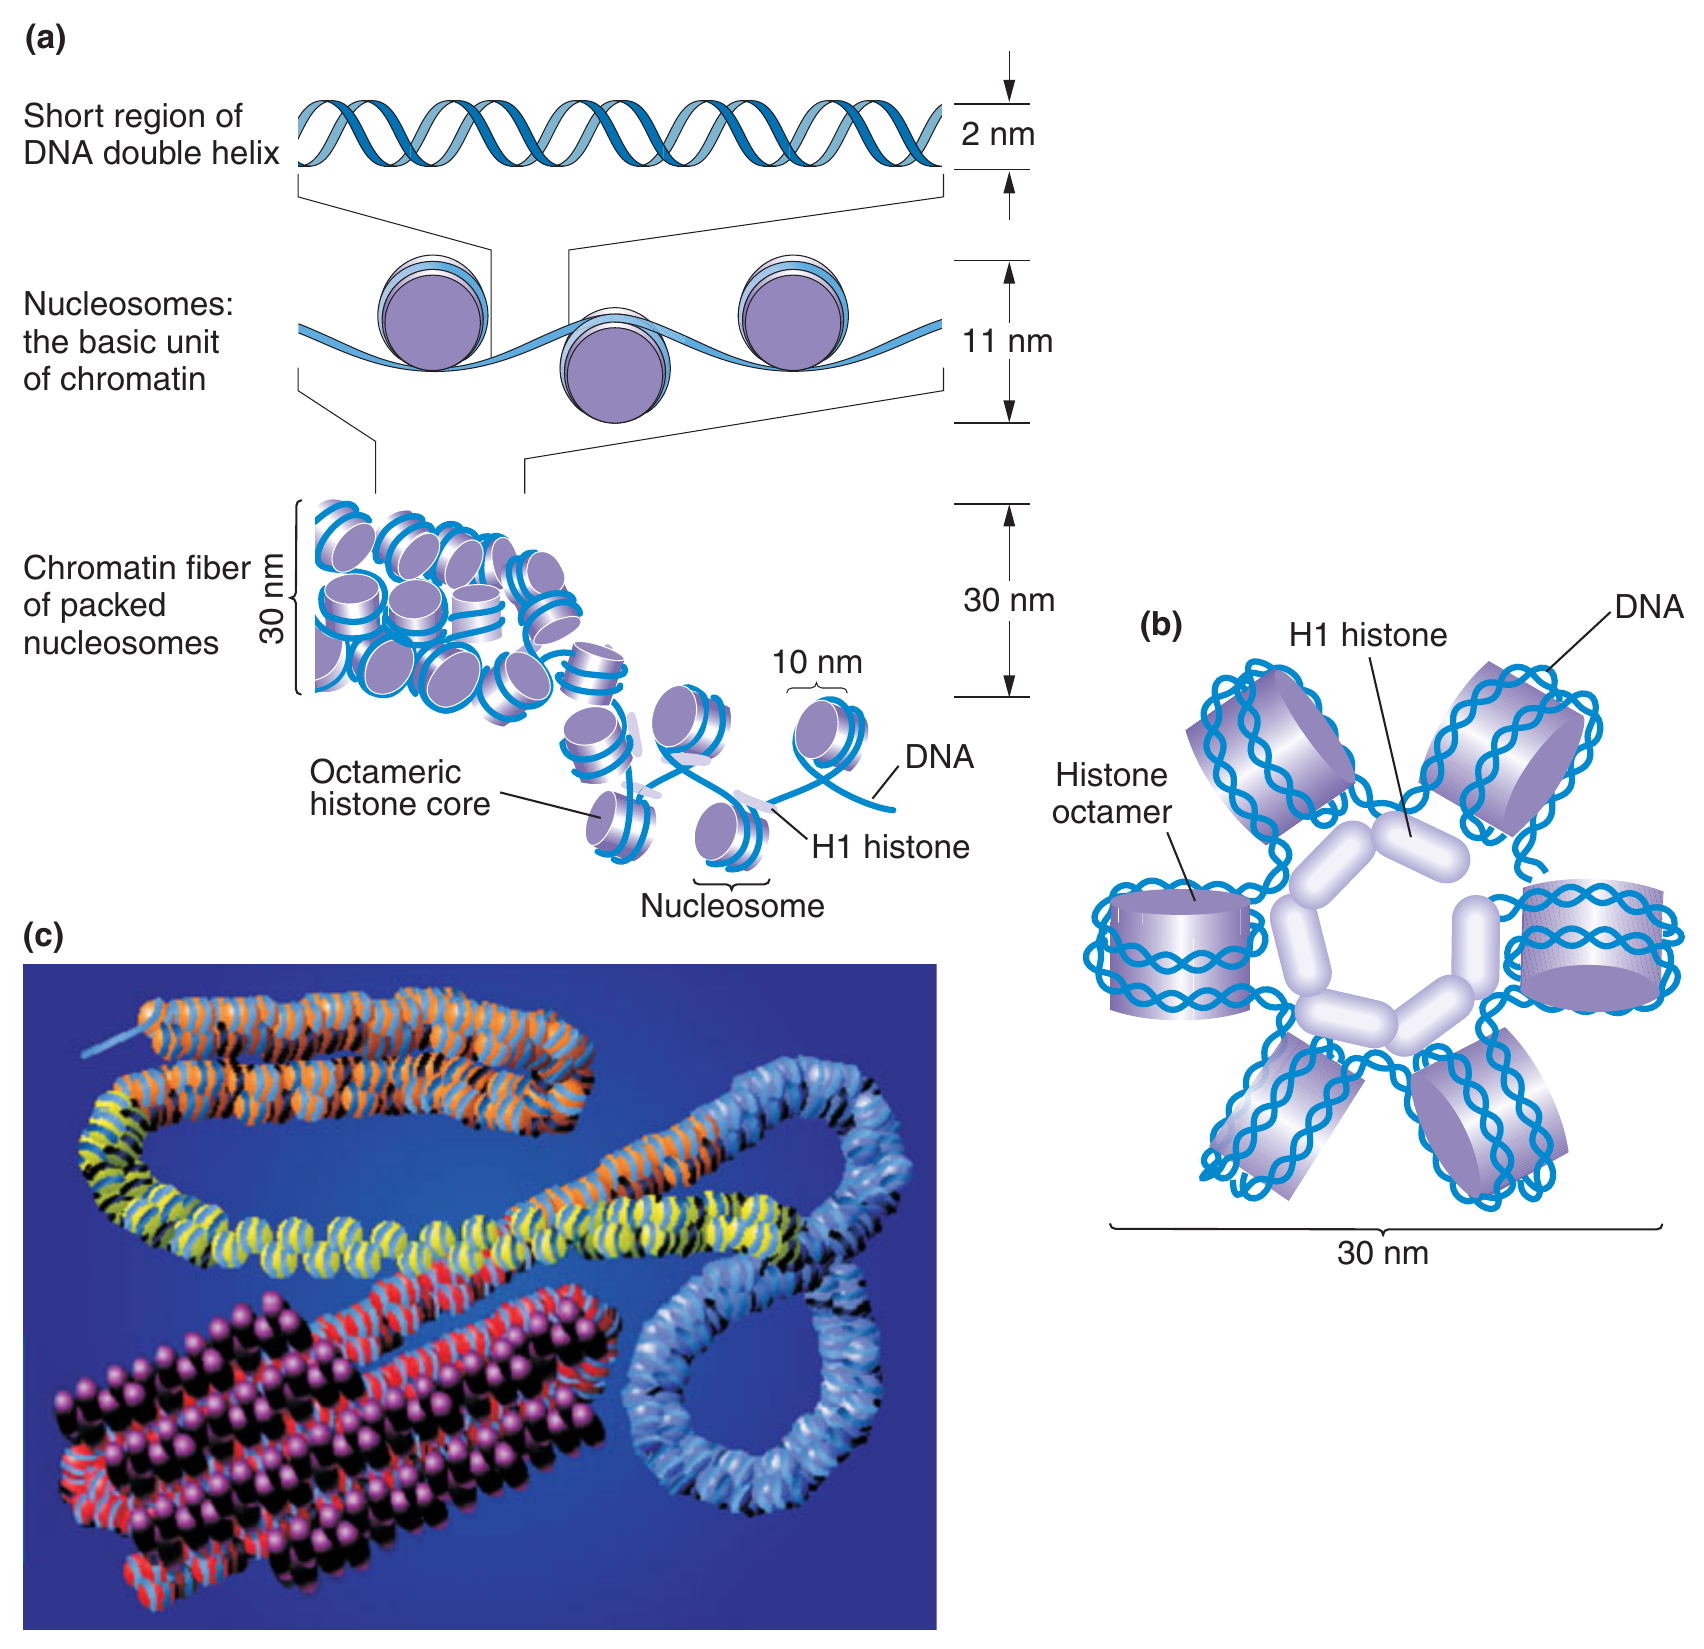
\includegraphics[width=0.45\linewidth]{../images/structure_of_chromatin} 

}

\caption{\textbf{Structure of chromatin} \newline (a) The nucleosome in decondensed and condensed chromatin. (b) End view of the coiled chain of nucleosomes. (c) Chromatin structure varies along the length of a chromosome. The least-condensed chromatin (euchromatin) is shown in yellow, regions of intermediate condensation are in orange and blue, and heterochromatin coated with special proteins (purple) is in red.}\label{fig:structure-of-chromatin}
\end{figure}
\end{frame}

\begin{frame}{Histones and basic chromosome structure}
\protect\hypertarget{histones-and-basic-chromosome-structure}{}
\begin{itemize}
\tightlist
\item
  Proteins having molecular weight ranging 10000-30000.
\item
  Completely deviod of tryptophan.
\item
  Highly heterogeneous
\item
  H1 is lysine rich, H2A and H2B are slightly lysine rich annd H3 and H4
  are arginine rich.
\item
  H2A, H2B, H3 and H4 are involved in the structural organization of
  chromatin fibers, while fraction H1 holds together the folded
  chromatin fibers.
\item
  30 nm diameter chromatin fibers are the basic units of chromosome
  structure. Such organisation of chromatin fibers in chromosomes is
  best explained by the \textbf{folded-fiber model} of chromosome
  structure.
\end{itemize}
\end{frame}

\begin{frame}{Folded fiber model}
\protect\hypertarget{folded-fiber-model}{}
\begin{itemize}
\tightlist
\item
  Each chromatid contains a single enourmously long chromatin fiber,
  which folds in various ways to yield the metaphase chromosome
  structure.
\item
  DNA of chromatin fiber replicates during interphase producing two
  sister chromatin fibers, except for centromeric region which undergoes
  replication during later stages of cell division.
\item
  During cell division, two sister chromatin fibers undergo extensive
  folding separately in an irregular but identifiable manner to give
  rise to sister chromatids of a chromosome.
\item
  Folding of chromatin fibers drastically reduces their length and at
  the same time markedly increases their thickness and stainability
  (that of euchromatin).
\item
  This folded structure normally undergoes supercoiling, which further
  reduces the length and increases chrnomosome thickness.
\end{itemize}
\end{frame}

\begin{frame}{}
\protect\hypertarget{section-11}{}
\begin{columns}[T,onlytextwidth]
  
  \column{0.5\textwidth}
  
\begin{figure}
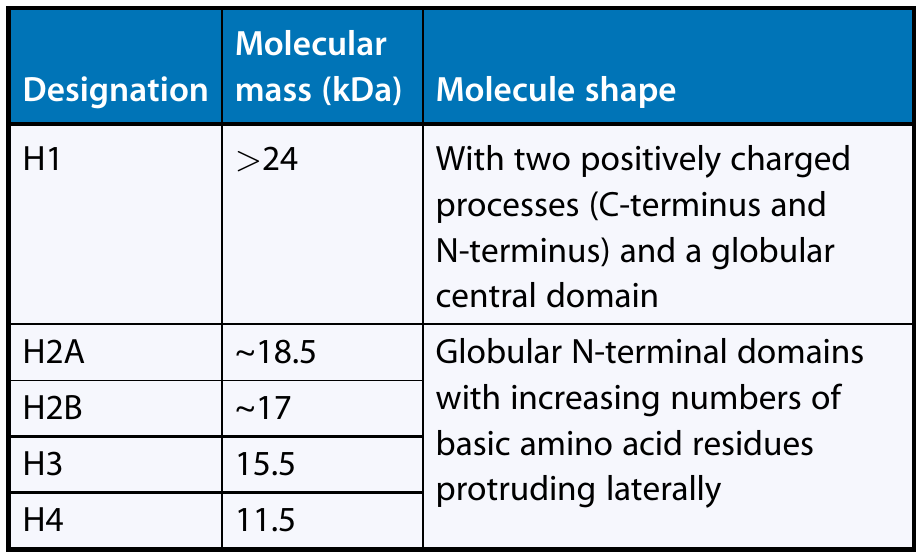
\includegraphics[width=0.65\linewidth]{../images/histone_types} \caption{Overview of five basic types of histone}\label{fig:histone-types}
\end{figure}

  \column{0.5\textwidth}

\begin{figure}
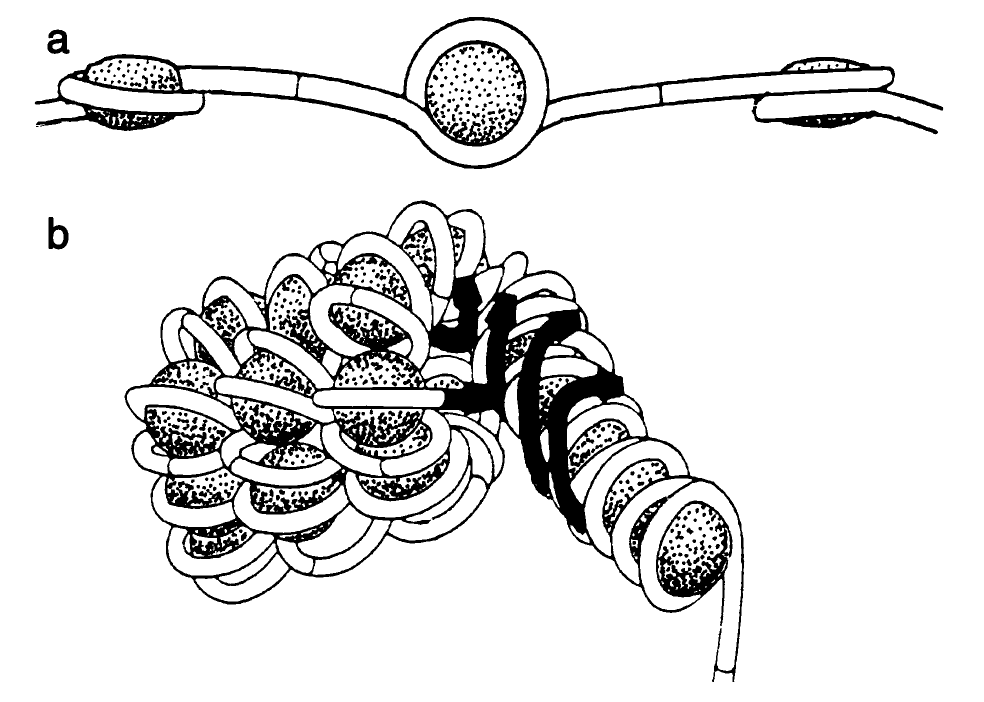
\includegraphics[width=0.8\linewidth]{../images/nucleosome_structure} \caption{\textbf{Nucleosomes}. (a) Beaded pattern: three histone octamers (dotted) surrounded by left-handed DNA double helices bonded by DNA linkers; horizontal stripes attack sites of Micrococcus nuclease. (b) Supranucleosomal structures, mediated by H1 (black); on the right nucleofilaments, on the left chromatin fibrils (H1 not is illustrated here)}\label{fig:nucleosome-structure}
\end{figure}

\end{columns}
\end{frame}

\begin{frame}{Packing of DNA into chromatin fiber: Nucleosome solenoid
model}
\protect\hypertarget{packing-of-dna-into-chromatin-fiber-nucleosome-solenoid-model}{}
\small

\begin{itemize}
\tightlist
\item
  The basic unit of chromatin is the nucleosome, a complete unit of
  which contains \textasciitilde150 bp of DNA wrapped 1.7 times around a
  core of histone proteins, and H1 histone.
\item
  The nucleosome core contains 8 histones, two subunits of each of the
  four histones: histones 2A, 2B, 3, and 4 (called H2A, H2B, H3, and H4)
  organized as two dimers of H2A and H2B and a tetramer of H3 and H4.
\item
  Linker histone, H1, surrounds the nucleosome core which can compact
  the nucleosomes into higher-order structures that further condense the
  DNA
\item
  The four histones H2A--H4, which have similar molecular sizes and
  shapes, automatically form (even without DNA) flat-ellipsoid
  quaternary structures.
\item
  In these particles, with diameters of up to 10 nm and thicknesses of 5
  nm, two molecules of every histone type are involved -- \emph{histone
  octamers}, made up of core histones.
\item
  The edge of the histone octamer is flatly encircled by a 145-bp-long
  sequence of DNA, marking the location of the particularly basic
  N-termini of the histone molecule (Shown in Figure
  \ref{fig:nucleosome-structure}).
\item
  The approximately 60-bp intermediate \textbf{linker} represents the
  preferred attack site for endonucleases. Thus, cleavage events attack
  uniform nucleohistone complexes of the same particle mass, the
  nucleosomes.
\end{itemize}
\end{frame}

\begin{frame}{}
\protect\hypertarget{section-12}{}
\small

\begin{itemize}
\tightlist
\item
  This changes when H1 is added. This molecularly heavier histone (also
  less conserved in evolutionary terms) is not involved in the
  construction of the histone octamers or nucleosomes but preferentially
  binds, using nonspecific sequences, to linker DNA and densely binds
  nucleosomes to histone octamers already occupied by DNA. This gives H1
  its other name of linker histone.
\item
  It causes the chromatin to condense; increasing amount of H1 makes the
  molecule even more compact.
\item
  Initially, nucleofilaments (elementary or fundamental fibrils) form
  with diameters of 10 nm; further condensation results in
  superstructures, e.g., solenoids (helix structures with six
  nucleosomes per turn; from greek \emph{solen} tube) regular zigzag
  structures, or supranucleosomal granula (nucleomeres).
\item
  Finally, the chromatin fibril is formed, a 35-nm-thick filamentous
  structure. The DNA double helix packed into the chromatin fibril would
  be more than 20 times as long were it to be in its uncondensed form.
\end{itemize}
\end{frame}

\hypertarget{genetic-control-mechanism-in-eukaryotes}{%
\section{Genetic control mechanism in
eukaryotes}\label{genetic-control-mechanism-in-eukaryotes}}

\begin{frame}{When should the academic month of an year start ?}
\protect\hypertarget{when-should-the-academic-month-of-an-year-start}{}
\centering \Huge \textbf{AUG}ust

\normalsize

(For an introductory overview of regulation of gene expression in both
prokaryotes and eukaryotes, refer to lecture slides on Gene Expression,
of Introductory Genetics in 1st Semester course.)
\end{frame}

\begin{frame}{}
\protect\hypertarget{section-13}{}
\begin{itemize}
\tightlist
\item
  Many features in single-celled and multicellular eukaryotes, are not
  found in bacteria and their viruses.
\item
  Geneticists and molecular biologists have discovered the functions of
  introns, RNA splicing, distant and multiple cis-acting regulatory
  elements, chromatin, alternative splicing, and, more recently, miRNAs.
\item
  Still, central to the genetic control of development is the control of
  differential gene expression.
\item
  Expressed proteins determines much of the cell's architecture, its
  enzymatic activities, its interactions with its environment, and many
  other physiological properties.
\item
  At a given time cell expressess only a fraction of the RNAs and
  proteins encoded in its genome. At different times, however, the
  profile of expression differs.
\end{itemize}
\end{frame}

\begin{frame}{Eukaryotic gene regulation takes place at two levels}
\protect\hypertarget{eukaryotic-gene-regulation-takes-place-at-two-levels}{}
\begin{itemize}
\tightlist
\item
  Transcriptional gene regulation
\item
  Post-transcriptional gene regulation
\end{itemize}
\end{frame}

\begin{frame}{Transcriptional gene regulation}
\protect\hypertarget{transcriptional-gene-regulation}{}
\begin{itemize}
\tightlist
\item
  If the final product is a protein, regulation could be achieved by
  controlling the transcription of DNA into RNA or the translation of
  RNA into protein.
\item
  The basic mechanism at work is that molecular signals from outside or
  inside the cell lead to the binding of regulatory proteins to specific
  DNA sites outside of protein-encoding regions, and the binding of
  these proteins modulates the rate of transcription.
\item
  These proteins may directly or indirectly assist RNA polymerase in
  binding to its transcription initiation site -- the \textbf{promoter}
  -- or they may \textbf{repress} transcription by preventing the
  binding of RNA polymerase.
\end{itemize}
\end{frame}

\begin{frame}{}
\protect\hypertarget{section-14}{}
\begin{itemize}
\tightlist
\item
  In general, the ground state of a bacterial gene is ``on.''
\item
  Unless there are repressor regulatory proteins nearby, RNA polymerase
  can directly bind to the DNA.
\item
  Activator regulatory proteins increase the binding of RNA polymerase.
\item
  However, the ground state of eukaryotic gene is ``off.''
\item
  The transcriptional machinery (including RNA polymerase II and
  associated general transcription factors) cannot bind to the promoter
  in the absence of other regulatory proteins.
\item
  Thus two main \textbf{features} of eukaryotic gene regulation system
  are:

  \begin{enumerate}
  \tightlist
  \item
    Ensure at any one time most genes in the genome is turned off
  \item
    Generate thousands of patterns of gene expression (diversity)
  \end{enumerate}
\end{itemize}
\end{frame}

\begin{frame}{}
\protect\hypertarget{section-15}{}
\begin{figure}
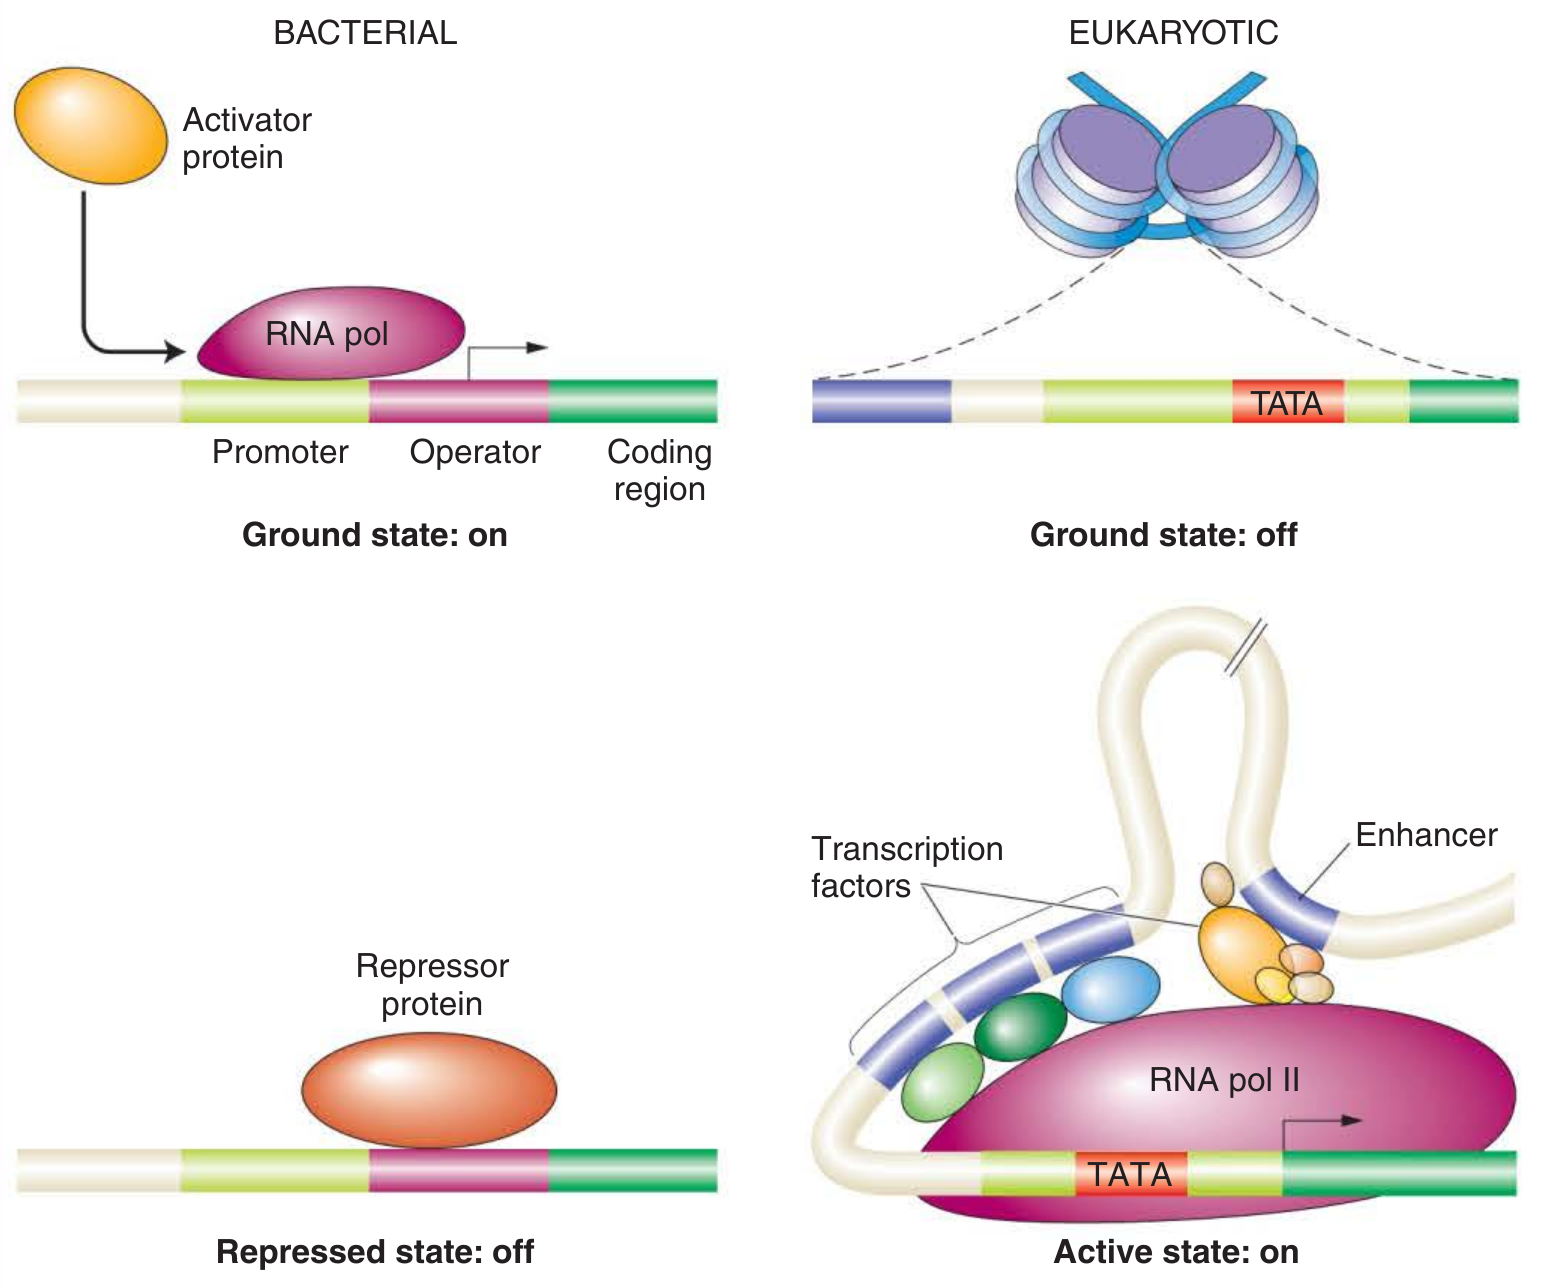
\includegraphics[width=0.65\linewidth]{../images/transcriptional_regulation} \caption{In bacteria, RNA polymerase can usually begin transcription unless a repressor protein blocks it. In eukaryotes, however, the packaging of DNA with nucleosomes prevents transcription unless other regulatory proteins are present. These regulatory proteins expose promoter sequences by altering nucleosome density or position. They may also recruit RNA polymerase II more directly through binding.}\label{fig:transcriptional-regulation}
\end{figure}
\end{frame}

\begin{frame}{Differences in transcriptional regulation of eukaryotes
and prokaryotes}
\protect\hypertarget{differences-in-transcriptional-regulation-of-eukaryotes-and-prokaryotes}{}
\begin{itemize}
\tightlist
\item
  In bacteria, all genes are transcribed into RNA by the same RNA
  polymerase, whereas three RNA polymerases function in eukaryotes.
\item
  RNA transcripts are extensively processed during transcription in
  eukaryotes; the \(5^\prime\) and \(3^\prime\) ends are modified and
  introns are spliced out.
\item
  RNA polymerase II is much larger and more complex than its bacterial
  counterpart. One reason it is more complex is that RNA polymerase II
  must synthesize RNA and coordinate the special processing events
  unique to eukaryotes.
\end{itemize}
\end{frame}

\begin{frame}{Eukaryotic transcription feature (2): Diversity of gene
expression pattern}
\protect\hypertarget{eukaryotic-transcription-feature-2-diversity-of-gene-expression-pattern}{}
\begin{itemize}
\tightlist
\item
  Includes trans acting regulatory \emph{proteins} and cis-acting
  regulatory DNA \emph{sequences}.
\item
  Two types of regulatory proteins based on the DNA regulatory sequences
  they bind:

  \begin{enumerate}
  \tightlist
  \item
    Large RNA polymerase II complex and general transcription factors;
    bind to promoter and act with cis-acting regulatory DNA sequences
    called \textbf{promoter-proximal elements}.
  \item
    Other transcription factors; bind to cis-acting regulatory sequences
    called enhancers (these may be located a considerable distance from
    gene promoters).
  \end{enumerate}
\item
  Much strategy hinges on how specific transcription factors control the
  access of general transcription factors and RNA polymerase II.
\end{itemize}
\end{frame}

\begin{frame}{}
\protect\hypertarget{section-16}{}
\begin{figure}
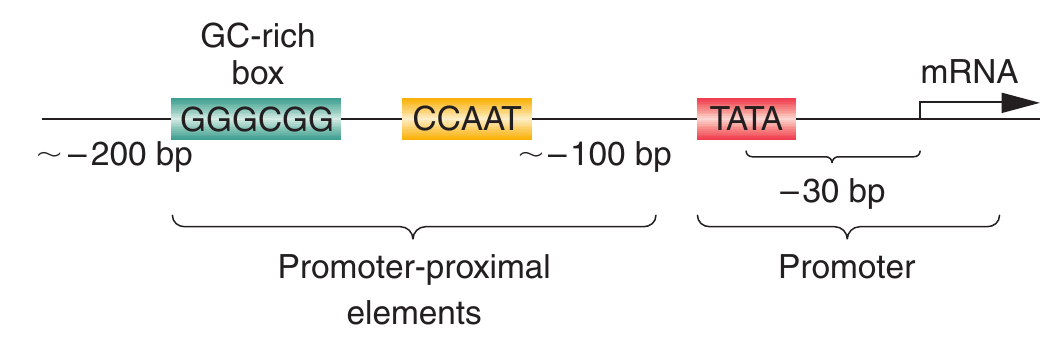
\includegraphics[width=0.65\linewidth]{../images/promoter_promoter_proximal_elements} \end{figure}
\end{frame}

\begin{frame}{}
\protect\hypertarget{section-17}{}
\begin{itemize}
\tightlist
\item
  Most studied gene regulatory system in eukaryote is that of Galactose
  metabolizing system (in \emph{Saccharomyces cerevisiae}).
\item
  Gal4 gene is the a characteristic of most transcriptional activators
  in eukaryotes (like Lac operon system of prokaryotes).
\item
  Similar to Gal4, many eukaryotic transcriptional regulatory proteins
  are modular proteins, having separable domains for DNA binding,
  activation or repression, and interaction with other proteins.
\item
  The activity of eukaryotic tanscriptional regulatory protein is often
  controlled by interactions with other proteins.
\item
  Eukaryotic transcriptional activators often work by recruiting parts
  of the transcriptional machinery (\textbf{mediator complex}; broadly
  called \textbf{co-activator}) to gene promoters.
\item
  The ability of Gal4, as well as other eukaryotic regulators, to
  function in a variety of eukaryotes indicates that eukaryotes
  generally have the transcriptional regulatory machinery and mechanisms
  in common.
\end{itemize}
\end{frame}

\begin{frame}{}
\protect\hypertarget{section-18}{}
\begin{figure}
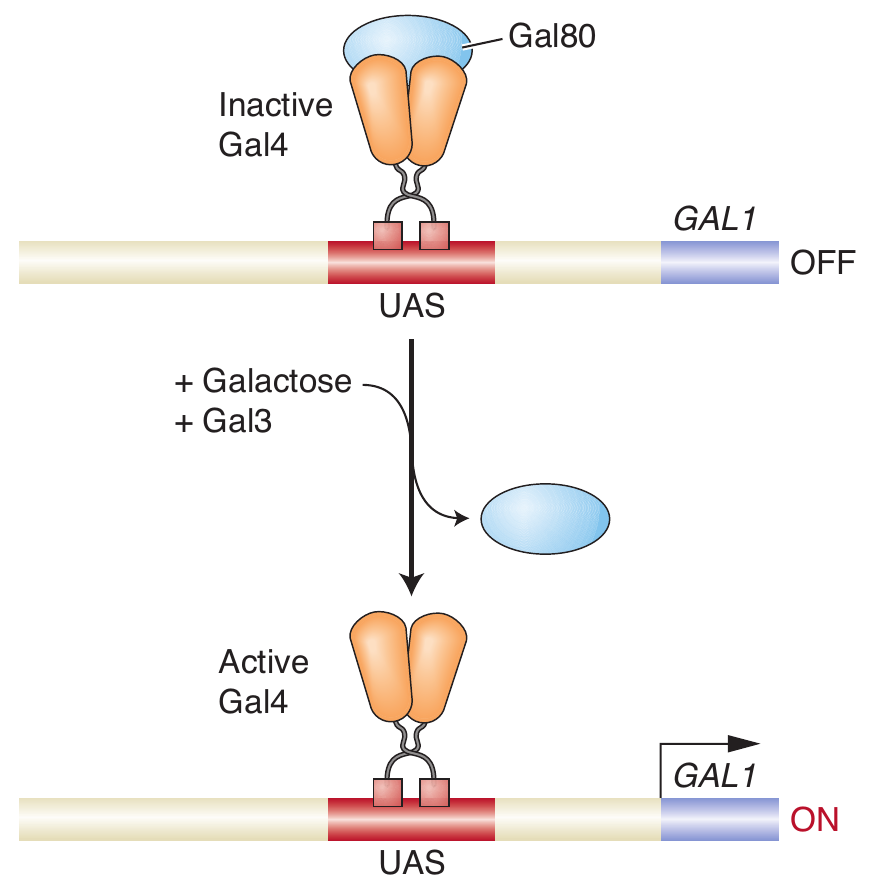
\includegraphics[width=0.4\linewidth]{../images/transcriptional_activator_proteins_inducer} \caption{\textbf{Transcriptional activator proteins may be activated by an inducer} \newline Gal4 activity is regulated by the Gal80 protein. (Top) in the absence of galactose, the Gal4 protein is inactive, even though it can bind to sites upstream of the GAL1 target gene. Gal4 activity is suppressed by the binding of the Gal80 protein. (Bottom) in the presence of galactose and the Gal3 protein, Gal80 undergoes a conformational change and is released, allowing the Gal4 activation domain to activate target gene transcription.}\label{fig:inducer-proteins}
\end{figure}
\end{frame}

\begin{frame}{Eukaryotic transcription feature (1): Dynamic chromatin}
\protect\hypertarget{eukaryotic-transcription-feature-1-dynamic-chromatin}{}
\begin{itemize}
\tightlist
\item
  A second mechanism for influencing gene transcription in eukaryotes
  modifies the local chromatin structure around gene regulatory
  sequences.
\item
  The modification of chromatin structure is a distinctive feature of
  many eukaryotic processes including gene regulation.
\item
  There are three major mechanisms to alter chromatin structure:

  \begin{enumerate}
  \tightlist
  \item
    moving nucleosomes along the DNA, also called chromatin remodeling.
  \item
    histone modification in the nucleosome core
  \item
    replacing the common histones in a nucleosome with histone variants.
  \end{enumerate}
\item
  Chromatin remodeling changes nucleosome density or position and is an
  integral part of eukaryotic gene regulation.
\end{itemize}
\end{frame}

\begin{frame}{}
\protect\hypertarget{section-19}{}
\begin{figure}
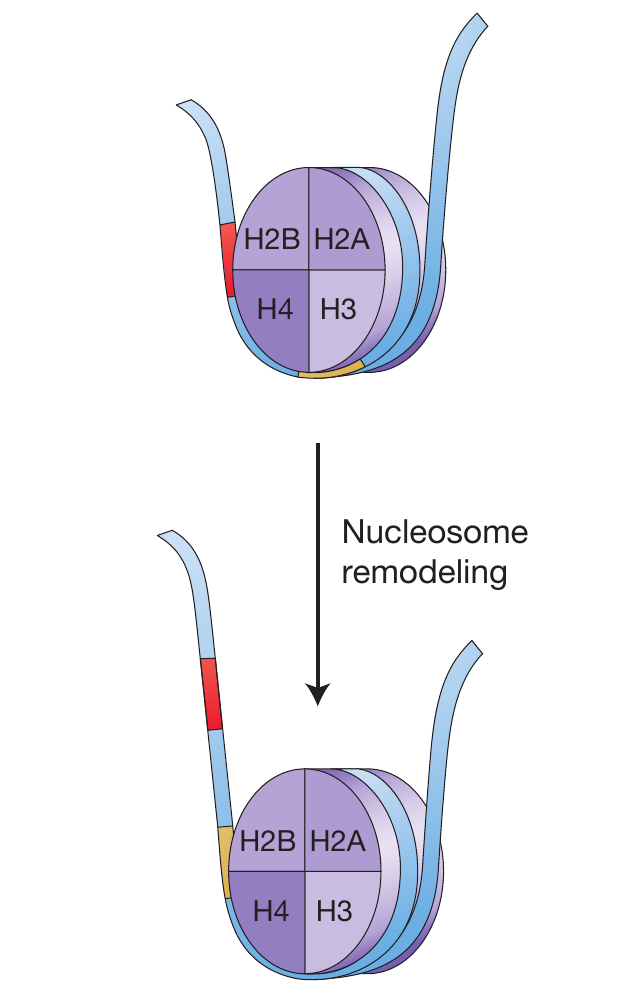
\includegraphics[width=0.3\linewidth]{../images/chromatin_remodeling} \caption{The histone octamer slides in response to chromatin-remodeling activity (such as that of the SWI–SNF complex), in this case exposing the DNA marked in red.}\label{fig:chromatin-remodeling}
\end{figure}
\end{frame}

\hypertarget{bibliography}{%
\section{Bibliography}\label{bibliography}}

\begin{frame}{References}
\protect\hypertarget{references}{}
\end{frame}




\end{document}
